\section{Model}
\label{sec:model}

This section formalizes the online scheduling problem for Large Language Model (LLM) inference under memory constraints. Unlike traditional scheduling, this task involves dynamically evolving resource demands due to the growing Key-Value (KV) cache and a two-phase (prefill and decode) processing structure. We first introduce the inference process, then describe prompt characteristics, batching rules, system constraints, and performance metrics.

\subsection{Prompts and Inference Process}

We analyze a system designed to process user queries, referred to as \textit{prompts}, utilizing a single Graphics Processing Unit (GPU) for computation. We focus on maximizing the utilization of single GPU and our algorithms can be extended to multi-GPU settings such as those utilizing pipeline parallelism, where each prompts are processed on different GPU in different layers on LLM model. Additionally, when there is no communication cost 
% (e.g. \cite{jaillet2025onlineschedulingllminference})
, our algortihms can generalize naturally to this setting as well. 

During the inference process, each prompt is divided into discrete units known as \textit{tokens} during the prefill phase and generates output text through an inference process in the decode phase. A token represents a distinct text element, such as a word or subword, and its processing relies on a memory structure called the Key-Value (KV) cache. As noted in the introduction, the KV cache improves inference efficiency significantly by storing the computational history of prior tokens, thus avoiding redundant computations. The cache size increases as tokens are processed, requiring careful memory management to maintain system performance.

% A Central Processing Unit (CPU) with unlimited memory acts as auxiliary storage; however, transferring a token’s KV cache from the CPU to the GPU introduces a delay \( d_s > 0 \) per token.

% \textbf{Prompt Characteristics}: Prompts arrive stochastically and are classified into \( m \) distinct types, indexed by \( j \in \{1, \dots, m\} \). A prompt of type \( j \) has the following properties:
% \[
% \begin{cases}
% \text{a length of } l_j \text{ tokens after completing the prefill phase;} \\
% \text{a length of } l_j + l_j' \text{ tokens after completing the decode phase.}
% \end{cases}
% \]
% We assume that prompts of type \( j \) follow a Poisson process with a rate of \( \lambda_j \).

% \gan{I will add more explanation. The rate $\lambda_j$ comes from the real world inference serving data, and the rate of one type is indeed the sum of rates of many mini types in the real world inference serving data. Or maybe this part should add to the nested WAIT section?}

\textbf{Prompt Characteristics}: Prompts arrive stochastically and are classified into \( m \) distinct types according to their input / output lengths, indexed by \( j \in \{1, \dots, m\} \). We assume that prompts of type \( j \) arrive according to a Poisson process with rate \( \lambda_j \) (however, our algorithms and analysis can be extended to more general cases with varying arrival rates, which is left in Appendix \ref{sec:extension}). A prompt of type \( j \) has the following properties:
\begin{equation*}
    \left\{
    \begin{aligned}
        &\text{a length of } l_j \text{ tokens after prefill;}\\
        &\text{a length of } l_j + l_j' \text{ tokens after decode.}
    \end{aligned}
    \right.
\end{equation*}
Therefore, a type-$j$ prompt must undergo one prefill iteration followed by $l_j'$ decode iterations to complete its inference processing. During the prefill phase, the prompt’s input context and question are embedded as $l_j$ tokens in a single iteration, consuming a KV cache of size $l_j$ units. In the subsequent decode phase, one output token is generated per iteration, each incurring an additional unit of KV cache memory. For clarity of exposition, we define a prompt to be in \textbf{stage 0} if it is about to undergo the prefill phase, and in \textbf{stage $k$} if it is scheduled to receive its $k$-th output token during the decode phase. Though the total number of different types can be large (for example, from $1$ to $10000$), as we will demonstrate later in this paper, our algorithms and their theoretical guarantees exhibit only a weak (logarithmic) dependence on \( m \), relying primarily on the total arrival rate across all types. This dependence on the total arrival rates ensures that our approach scales efficiently across various operational scenarios, regardless of the number of types. Moreover, while our analysis focuses on fixed arrival rates \( \lambda_j \), our threshold-based algorithms can be extended to settings with time-varying arrivals by dynamically adjusting the thresholds based on the arrival rates.


% The uncertainty of the output length distinguishes our model fundamentally from previous work, such as \cite{jaillet2025onlineschedulingllminference}, which assumes known output lengths. 

\subsection{Batching and GPU Processing Dynamics}
To optimize resource utilization, the GPU processes tasks in \textit{batches}, combining prompts for prefilling and prefilled prompts for decoding. Figure~\ref{fig:batching_example} illustrates the temporal dynamics of batching and scheduling in GPU-based inference. Two prompts, \( P1 \) and \( P2 \), arrive sequentially and are processed according to their current stage—prefill or decode—at each time step. Initially, \( P1 \) arrives and enters the prefill phase, embedding its input sequence ``How are you?'' in a single iteration. Shortly after, \( P2 \) arrives with the query ``Is 5 a prime?'', which is also scheduled for prefill. The GPU batches prompts in the same phase together; thus, \( P1 \) is processed for prefill alone, followed by \( P2 \). At the next step, \( P1 \) enters the decode phase, generating its first output token ``I'm,'' while \( P2 \) undergoes prefill in parallel. Subsequently, both prompts advance in the decode phase, each generating one token per iteration: ``Yes'' for \( P2 \) and ``I'm fine'' for \( P1 \). This example highlights how the scheduler interleaves prompts in different stages—prefill and decode—into shared GPU batches, thereby improving throughput. Importantly, prefill stages involve initializing KV caches based on input tokens, while decode stages extend outputs one token at a time, with incremental KV cache updates.


In general, consider a batch composed of:
\begin{itemize}
    \item \( n_1 \) prompts in the prefill phase, each with an input length of \( k_i \) tokens for \( i = 1, 2, \dots, n_1 \). These prompts are processed to initialize their KV caches.
    \item \( n_2 \) prompts in the decode phase, each with output length of \( s_i = l_{j(i)} + k_i \) tokens after the current iteration, where \( l_{j(i)} \) is the input length of prompt \( i \) of type \( j(i) \), and \(1\le k_i \le l_j'\) denotes the number of tokens generated so far in the decode phase for prompt \( i \).
\end{itemize}


\begin{figure}[h]
    \centering
    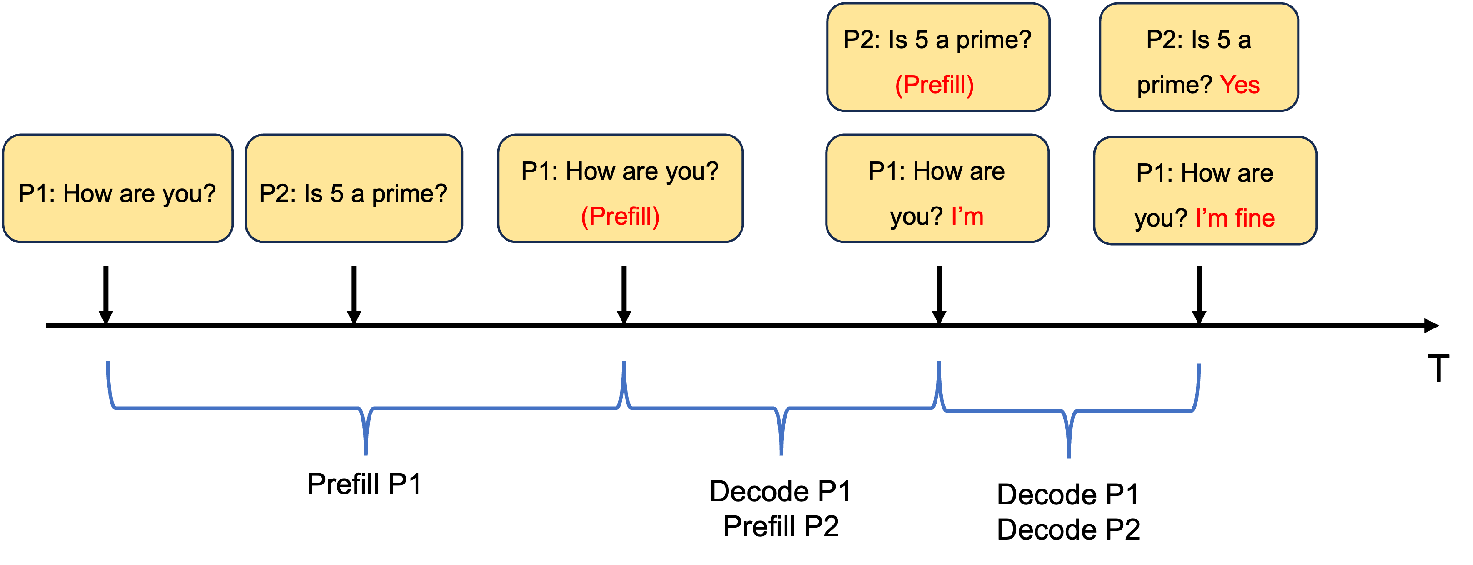
\includegraphics[width=0.6\linewidth]{Experiments_pdf/fig_batching1.pdf}
    \caption{Example of batching and scheduling.}
    \label{fig:batching_example}
\end{figure}

Based on experimental results from \cite{agrawal2023sarathi,kwon2023efficient,zhong2024distserve}, we model the \textit{iteration time} to process a batch as:
\begin{equation}
\label{eq:time_consump}
    \tau = d_0 + d_1 \cdot \left( \sum_{i=1}^{n_1} k_i + \sum_{i'=1}^{n_2} s_{i'} \right),
\end{equation}
where \( d_0 \) denotes the fixed overhead time associated with processing a batch, and \( d \) represents the time cost per unit of memory. This formulation indicates that the iteration time for each batch scales linearly with the total memory utilization, reflecting the direct dependence of computational latency on memory consumption involving reading existing KV cache and computing the new one. Figure \ref{fig:inference time} provides a numerical validation of this modeling. We deploy Llama-7B and Llama-13B on a single L20 GPU to test time cost per-iteration, using batches consisting of different number of tokens with 20 repeats. The result is highly in accordance with our model. An important observation is, as $d_1 \cdot \left( \sum_{i=1}^{n_1} k_i + \sum_{i'=1}^{n_2} s_{i'} \right)/[d_0 + d_1 \cdot \left( \sum_{i=1}^{n_1} k_i + \sum_{i'=1}^{n_2} s_{i'} \right)]$ increases, the more memory per iteration is used and the more efficient the LLM inference process.

\begin{figure}
    \centering
    
\includegraphics[width=0.6\linewidth]{Experiments_pdf/inference_time_comparison.pdf}
    \caption{Inference time of Llama-7B and Llama-13B with different number of tokens in the batch on a single L20 GPU}
    \label{fig:inference time}
\end{figure}

\subsection{Constraints and Performance Metrics}

\textbf{Memory Constraint}: At every batch iteration $t$, the total memory usage must not exceed GPU capacity $C$:
\[
\sum_{i \in B^t} (l_{j^t(i)} + k^t_i) \le C,
\]
where $B^t$ is the batch set at iteration $t$, $j^t(i)$ is the prompt type, and $k^t_i$ is its current processing stage.

\textbf{Performance Metrics}: We define clearly the metrics guiding scheduling optimization:
\begin{itemize}
    \item \textbf{Throughput}: Average number of tokens generated in decode phase per unit time, measuring system efficiency. The throughput for a prompt is counted only after it is completed to ensure validity of the output.
    \item \textbf{Latency}: Average elapsed time from prompt arrival to completion, capturing responsiveness.
    \item \textbf{Time to First Token (TTFT)}: Average delay from prompt arrival to the generation of the first token, reflecting initial user-perceived delay.
\end{itemize}

\subsection{Optimization Problem}
We formalize the problem as optimizing throughput subject to latency and TTFT constraints over continuous time horizon $[0,T]$:
\begin{equation*}
    \begin{aligned}
            \max_{\pi \in \Pi} \quad &\ex{}{\throughput^{(T,\pi)}}, \\
    \text{s.t.}\quad & \ex{}{\Latency^{(T,\pi)}} \le L^T,\\
    & \ex{}{\TTFT^{(T,\pi)}} \le F^T, \\
    & \sum_{i \in B^t} (l_{j^t(i)} + k^t_i) \le C \quad \forall t,
    \end{aligned}
\end{equation*}
where $\Pi$ denotes admissible non-preemptive scheduling policies. Preemption—pausing and later resuming ongoing prompts—is allowed. However, due to substantial overhead costs incurred from KV cache recomputation, we allow the policy to hold the computed KV caches on GPU but pause certain jobs temporarily. 
% This formulation
% encapsulates the potential trade-offs between resource efficiency and service quality: without the latency and TTFT constraints, the algorithm may always prioritize the shortest jobs in order to maximize the throughput and the latency of the long jobs can be very large in overloaded systems.

% \subsection{Unique Challenges and Comparison to Prior Work}

% This model poses distinct analytical and operational challenges not addressed by conventional scheduling literature:
% \begin{enumerate}
%     \item \textbf{Dynamic memory growth}: Unlike traditional jobs, prompts exhibit progressively increasing memory usage during decoding, complicating classical static memory allocation methods.
%     \item \textbf{Output length uncertainty}: Unlike Jaillet et al. (2025), which assumes known output lengths, our scenario reflects realistic settings where output predictions are unreliable, thus complicating analysis and batch formation strategies.
%     \item \textbf{Multi-stage process}: Prefill and decode phases differ significantly in computational patterns, necessitating a fluid approximation approach to handle their differing resource demands analytically.
% \end{enumerate}

% To address these challenges, we propose a fluid-based analytical framework and threshold-based policies (Sections~\ref{sec:fluid}-\ref{sec:nested_wait}) explicitly designed to operate efficiently under realistic conditions of output uncertainty and stochastic arrivals. This distinguishes our work analytically and practically from existing literature.
